\documentclass[10pt,letter]{article}
\usepackage[margin=1.0in]{geometry}

\usepackage{amsmath}
\usepackage{amssymb}
	% packages that allow mathematical formatting

\usepackage{graphicx}
	% package that allows you to include graphics

\usepackage{hyperref}
\hypersetup {
    colorlinks=true,
    urlcolor=cyan
}

\usepackage{setspace}
	% package that allows you to change spacing

\onehalfspacing
	% text become 1.5 spaced

\newcommand{\horrule}[1]{\rule{\linewidth}{#1}} % Create horizontal rule command with 1 argument of height

\begin{document}
	% line of code telling latex that your document is beginning

\horrule{1pt}
\begin{center}
\section*{NENS 230\\ Assignment \#7}
Statistics and Hypothesis Testing\\
Due: Tuesday, November 10th, 2015
\end{center}
\horrule{1pt}

\section*{Goals}
\begin{itemize}
    \item Learn the basic application of statistics and hypothesis testing using MATLAB
    \item Use MATLAB to perform statistical testing (T-test) on behavioral data.
\end{itemize}

\section*{Problem 1: Using statistics in MATLAB}

\subsection*{Tutorial}

In this first section you will complete the statistics tutorial \texttt{statistics-tutorial.m}, which takes you through sections of code that touch upon various topics in hypothesis-driven statistics. This isn't a problem in the sense that you will not be writing any code for this problem, but there are questions to go along with each part of the tutorial which you will need to answer. They are more conceptual as the aim is for you to understand the tutorial. Please submit your answers as a text file named \texttt{tutorial-answers}.

\section*{Problem 2: Statistical testing on behavioral data}

\subsection*{Introduction}

Neural plasticity, or the ability of neural circuits to change, is essential for both normal brain function and recovery from injury. After stroke, increased plasticity is associated with faster recovery. On the other hand, inflammation can impair plasticity and exacerbate damage. In a recent paper, researchers at Stanford tested whether mice that lacked certain immune system molecules might recover faster from a stoke (Adelson et al. 2012). 

One set of mice were missing the gene for PirB, an innate immune receptor for MHC molecules. In other mice, two of its ligands (MHCI Kb and Db) were deleted. These molecules are known to be upregulated during inflammation, and to limit synaptic plasticity in healthy brains. We will analyze some mock data to determine if PirB deletion improves motor recovery.

\subsection*{Hypothesis testing}

Let’s see if PirB deletion improves recovery from stroke. The provided Excel file contains data from mice walking across a horizontal ladder as a test of motor performance. When a paw slips through the ladder, a “foot fault” is recorded – fewer faults mean better performance. Figure 1C from the paper shows data on MHC1 KbDb knockout animals and is a good model for what your final plot should look like – here the MHCI knockouts have improved motor performance!


\begin{figure}[h!]
\centering
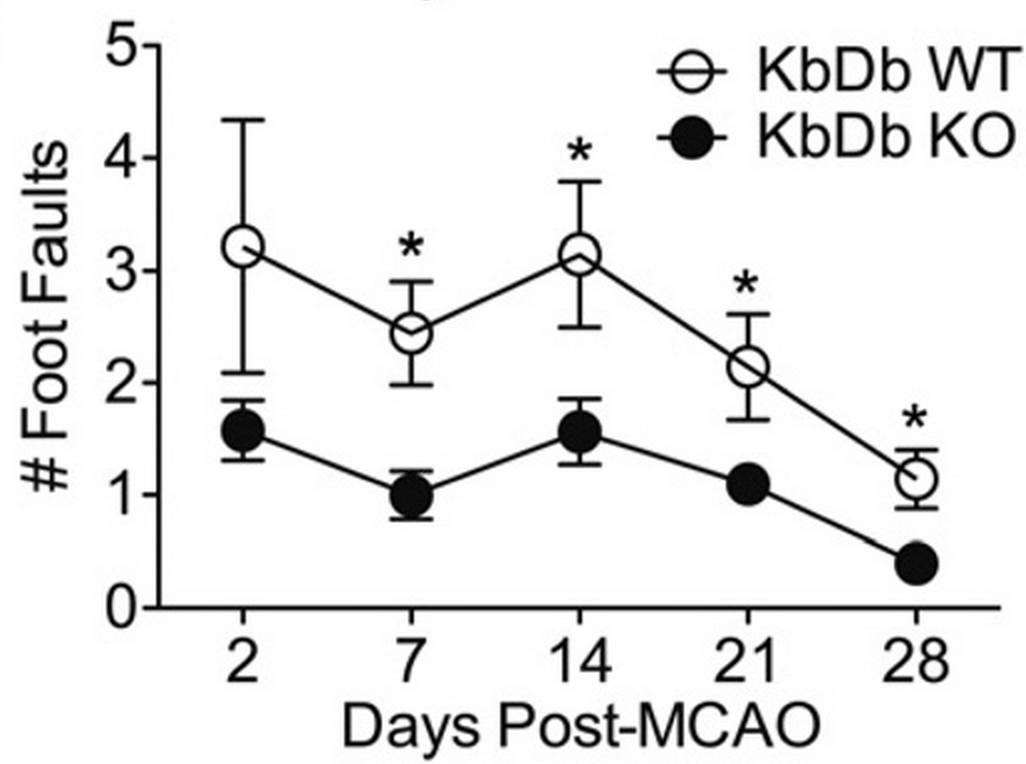
\includegraphics[width=0.6\textwidth]{footfaults.png}
\caption{  }
\label{fig:awesome_image}
\end{figure}


Name your script for this assignment \texttt{assignment7.m}. Load data from the provided Excel spreadsheet footfaults.xls using xlsread. Each column is a different time point, each row a different mouse. Worksheet 1 contains data from 8 control animals tested at 2, 7, 14, 21, and 28 days after stroke. Worksheet 2 contains data from knockout animals missing the gene for PirB. Plot a time series of control and mutant data. Include bar indicating standard error and label the x-axis with the correct day numbers.  You can use the provided \texttt{errorb()} function to add the error bars, but you'll need to calculate the standard error.


Test for significance at each time point, using a t-test with the standard significance level of 0.05 – but correct for multiple comparisons since the data at different time points are not independent! An easy way to do this is known as the Bonferroni correction (http://en.wikipedia.org/wiki/Bonferroni\_correction), in which you simply make each test more stringent by dividing the required p value by the number of comparisons. So to ensure an overall false-positive rate of 5\%, with comparisons at five time points, you would make the effective p-value 0.05 divided by 5. Since we are making 5 non- independent tests (one for each time point), we need to adjust the significance level by a factor of 5 to alpha = 0.01. If a time point is significant, plot a star at a fixed distance above the control error bar.  Your plot includes mock data which is different from that in the figure shown here, so don't worry if the plots don't look identical.  The general form, placement of the asterisks, etc. should be similar, however.  

Reference
Adelson et al. (2012). Neuroprotection from Stroke in the Absence of MHCI or PirB. Neuron, 73, 1100-7. 

\section*{Submission}
When you are finished, publish your work with the \texttt{publish} command. Email the generated PDF file, along with your code, to \texttt{nens230@gmail.com} with \texttt{[Assignment 7]} in the subject line to submit your assignment.

\end{document}
